\documentclass{sigchi}

% Use this command to override the default ACM copyright statement (e.g. for
% preprints).
% Consult the conference website for the camera-ready copyright statement.
\toappear{
	Robin Hahling and Kevin Gillieron\\
    licensed under CC BY-NC, 2013\\
    
\includegraphics[scale=0.5]{img/cc-by-nc.png}
}

% Arabic page numbers for submission.
% Remove this line to eliminate page numbers for the camera ready copy
\pagenumbering{arabic}


% Load basic packages
\usepackage{balance}  % to better equalize the last page
\usepackage{graphics} % for EPS, load graphicx instead
%\usepackage{times}    % comment if you want LaTeX's default font
\usepackage{url}      % llt: nicely formatted URLs

% llt: Define a global style for URLs, rather that the default one
\makeatletter
\def\url@leostyle{%
  \@ifundefined{selectfont}{\def\UrlFont{\sf}}{\def\UrlFont{\small\bf\ttfamily}}}
\makeatother
\urlstyle{leo}


% To make various LaTeX processors do the right thing with page size.
\def\pprw{8.5in}
\def\pprh{11in}
\special{papersize=\pprw,\pprh}
\setlength{\paperwidth}{\pprw}
\setlength{\paperheight}{\pprh}
\setlength{\pdfpagewidth}{\pprw}
\setlength{\pdfpageheight}{\pprh}

% Make sure hyperref comes last of your loaded packages,
% to give it a fighting chance of not being over-written,
% since its job is to redefine many LaTeX commands.
\usepackage[pdftex]{hyperref}
\hypersetup{
pdftitle={Mining tweets ti predict their popularity},
pdfauthor={Texlive},
pdfkeywords={datamining, twitter, tweet, classification, prediction, popularity},
bookmarksnumbered,
pdfstartview={FitH},
colorlinks,
citecolor=black,
filecolor=black,
linkcolor=black,
urlcolor=black,
breaklinks=true,
}

% create a shortcut to typeset table headings
\newcommand\tabhead[1]{\small\textbf{#1}}


% End of preamble. Here it comes the document.
\begin{document}

\title{Mining tweets to predict their popularity}

\numberofauthors{2}
\author{
  \alignauthor Robin Hahling\\
    \affaddr{University of Geneva,\\ Computer Science Department}\\
    \affaddr{Carouge, GE, CH}\\
    \email{hahlinr0@etu.unige.ch}\\
  \alignauthor Kevin Gillieron\\
    \affaddr{University of Geneva, Computer Science Department}\\
    \affaddr{Carouge, GE, CH}\\
    \email{gilliek0@etu.unige.ch}\\
}

\maketitle

\begin{abstract}
\textit{
In this paper we experiment several classifiers and features extracted from
tweets in order to predict if a tweet will be retwitted or not.
To do so, we analyzed data extracted from Twitter related to the keyword
"shampoo", thus related to a community around this theme.
Our approach focuses on extracting relevant features from tweets and using them
to train several different classifiers such as Support Vector Machine, Decision
Tree, Linear Discriminant Analysis, Maximum Entropy and Naive Bayes.
We validate our approach by performing a cross-validation and comparing the
classifiers in an algorithm tournament. The significance of our result is
validated by the McNemar test with Bonferroni adjustment.
Our result allows us to predict if a tweet will be retweeted with an accuracy 
over 94\%.
}
\end{abstract}

\section{Introduction}

Twitter is a microblogging system in which users cand send, reply, or forward
(retweet), short messages up to 140 characters between them. Typically, users
are inter-connected by messages and they form social network communities in
which different topics are discussed. Messages which are retweeted several times
are thus more likely to represent important topics that people like to discuss.
In this project, we analyzed twitter data and built models for solving 
the following task: to predict if a tweet will be retweeted or not, i.e. to 
predict if a tweet can be considered as popular or not insight a community.

To do so, we had to develop our own data mining tool and propose an
approach to solve the problem.

Our analysis was made on a recent collection of $42960$ tweets, all of which 
are related to the global topic of \textit{shampoo}. Due to the limitations of 
the new Twitter API v1.1, we were not able to fetch any more tweet than that. 
They cover a range of seven days (from the 13th of June to the 20th of June 
2013).

Each tweet is characterized by some features which we used, along with others 
we created, mostly built on the tweet's content, to compute our prediction.

Our approach was to first extract informative features from the tweets and then 
use them into various classifiers to do our prediction. We determined which 
features were the most informative and which classifier performed the best by 
doing algorithm tournament.
\section{Tools used}
\label{sec:tools}

\verb|Python| was our language of choice to implement our tool to predict if a 
tweet will be retweeted or not. Multiple libraries were used:
\begin{itemize}
	\item matplotlib: to plot 2D graphs of the ROC curve.
	\item nltk: for stemming and various language processing functions and some 
		  classifiers.
	\item numpy: to use special array objects.
	\item scipy: for some numerical routines.
	\item scikit-learn: for some classifiers.
	\item twython: to extract tweets from Twitter using their API.
\end{itemize}

Due to some libraries being not compatible with \verb|Python 3|, we had to 
stick with \verb|Python 2|.

We were able to develop a comprehensive tool that is easy to extend by taking 
advantage of object oriented programming. Adding new features or new 
classifiers can be done very easily thanks to the concept of inheritance.

The figure \ref{fig:architecture} shows the global architecture of the 
interesting part of the code.

\begin{figure}[!h]
\centering
 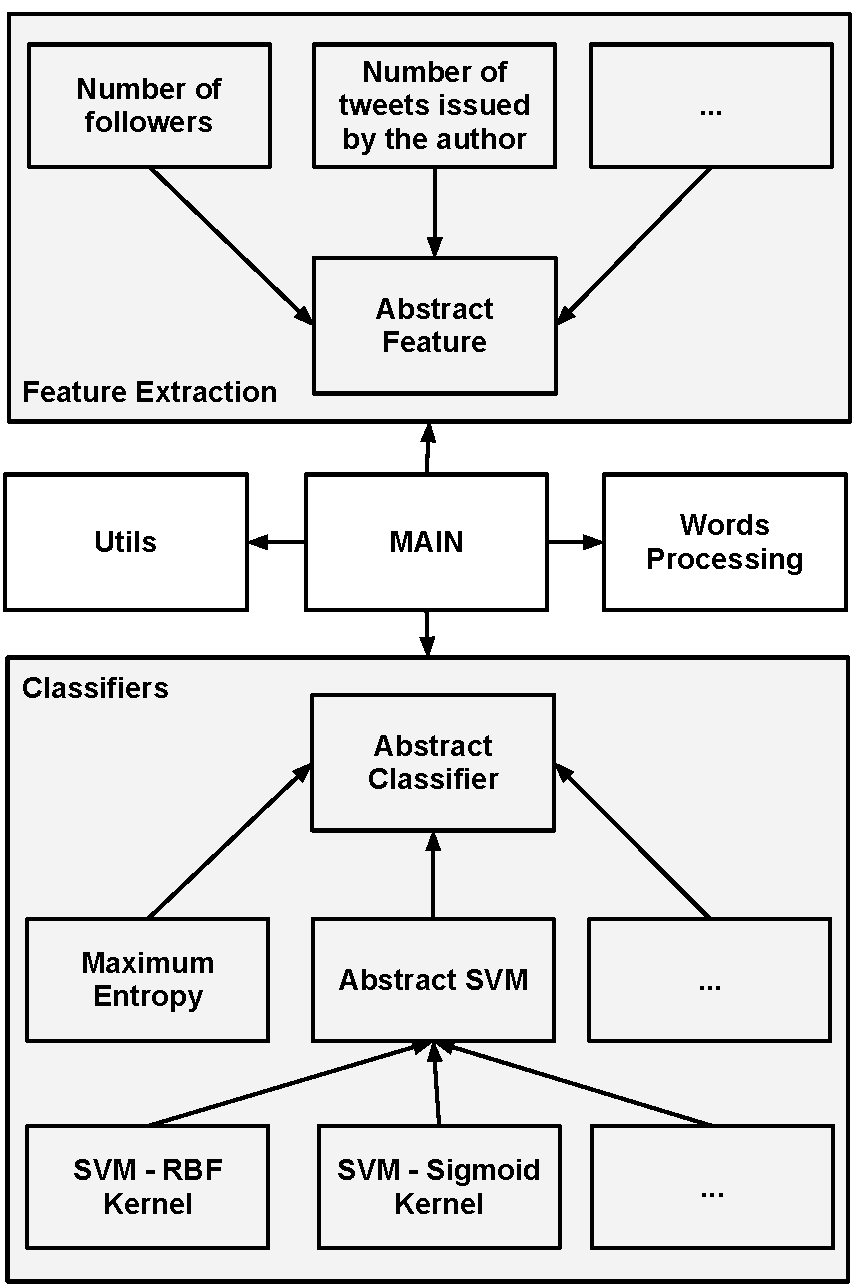
\includegraphics[width=0.9\columnwidth]{img/architecture.pdf}
\caption{Source code architecture}
\label{fig:architecture}
\end{figure}

Our tool is able to perform various tasks such as classification using numerous 
classifiers and features, algorithm tournament and cross-validation. It is also 
able to plot ROC curve and Decision Trees, randomizing the dataset and taking 
the advantage of multiprocessing for performing hard computing tasks.

In order to let the scientific community, or any people, use it, we released it 
under the terms of the permissive BSD license. Being written in \verb|Python|, 
it is available for any operating system on which \verb|Python| can run. We, 
however, only tested it on Linux.

\section{Dataset preparation}
\label{sec:dataset}

To analyze the tweets, we needed to collect a dataset of tweets.
We collected tweets related to the keyword \textit{shampoo}. Due to the
limitations of the free Twitter API, we were only able to collect tweets for a
recent period of time. The dataset comprises $42960$ tweets from which 
$59.78\%$ are retweets.

In order to extract some features, we had to do some preprocessing on the
dataset. To compute the term frequency - inverse document frequency, the
occurrence of words in the tweets needed to be computed.

To do so, we had to first create a corpus and then compute the occurrence of
each word. Only the text from the tweets was kept. Insignificant words were 
removed so that only nouns, verbs and adjectives were kept.We used Penn Treeban 
Part-of-Speech Tags for this task.  URLs, stop words or other special 
characters were obviously removed too. Once we had built the corpus, we created 
a file containing each words of the corpus and their occurrence throughout the 
whole dataset's tweet's text.

These words occurrences were later used in order to compute words frequencies 
used in TF and TF-IDF features.

The labels extracted from the tweets have an entropy of $0.97$.

\section{Features description}

In this section, we describe the features that are relevant for our work and 
mention the other features that have been removed from the final experiment. The 
table \ref{tab:features} lists all the features.

\begin{table}[!h]
 \centering
 \begin{tabular}{|c|l|}
  \hline
  \tabhead{\#} &
  \multicolumn{1}{|p{0.7\columnwidth}|}{\centering\tabhead{Features used}} \\
  \hline
  1  & is the tweet a retweet \\
  2  & is the tweet a reply \\
  3  & number of followers \\
  4  & number of times "favorited" \\
  5  & number of tweets issued by the author \\
  6  & is the author a verified account \\
  7  & number of user's friends \\
  8  & number of hashtags \\
  9  & number of words in the tweet \\
  10 & number of users mentionned \\
  11 & has an URL \\
  12 & TF feature \\
  13 & tweet's age \\
  14 & TF-IDF feature \\
  \hline
 \end{tabular}
 \caption{This table lists the features used in our work. Their order has no 
  specific meaning.}
 \label{tab:features}
\end{table}

The first feature indicates if a tweet is a retweet or not. This information is 
extracted from the text of the tweet which appears as a citation of the 
original tweet with the form "RT @username:". 

The feature number 2 determines whether a tweet is a reply to another 
tweet.This information is provided by the attribute "in\_reply\_to\_user\_id" 
which contains a non-null value if the tweet is a reply.

The third feature counts the number of followers the author has. This value 
is given by the \emph{User} object attached to a tweet.

The feature number 4 indicates how many times a tweet has been "favorited" by 
other users. This count is given by the attribute "favorite\_count"  of a tweet 
object.

The fifth feature gives the number of other tweets (including retweets) issued 
by the author. This information is provided by the attribute "statuses\_count" 
of the \emph{User} object.

The feature number six indicates if the author of the tweet has a verified 
account. Such accounts establish the authenticity of the user's identity. In 
our case, this means that the author of the tweet is famous and then he will be 
probably retweeted.

The seventh feature is the number of friends (aka the number users following 
the author). This count is provided by the \emph{User} object. The number of 
friends is strongly related to the number of retweets.

The feature number eight counts the number of hashtags from the \emph{Tweet} 
object and the feature number nine is the number of words of the tweet.

The tenth feature gives the number of users mentionned with a "@username" in 
the tweet. This information is calculated from the list of "user\_mentions" 
given by the \emph{User} object.

The feature number eleven indicates if the tweet contains an URL or not. The 
list of URL is provided by the \emph{Tweet entities} object.

Since the three last features did not give good results, they have been 
removed. The TF (Term Frequency) and the Tweet age were not significant while 
the TF-IDF (Term Frequency - Inverse Document Frequency) feature did not work 
due to a bug in the \emph{scikit} library.
\section{Classifiers}
\label{sec:classifiers}

In this work, we used and compared the 5 following classifiers :

\begin{itemize}
 \item Naive Bayes \cite{jurafsky2000speech}, \cite{kalousis2013}
 \item {Support Vector Machine (SVM) \cite{cristianini2000introduction},
	\cite{kalousis2013}
	\begin{itemize}
	 \item with a RBF Kernel
	 \item with a Sigmoid Kernel
	\end{itemize}}
 \item Maximum Entropy (MaxEnt)\cite{jurafsky2000speech}
 \item Decision Tree \cite{kalousis2013}
 \item Linear Discriminant Analysis (LDA) \cite{kalousis2013}
\end{itemize}

We excluded the Support Vector Machine from the cross-validation and 
the algorithm tournament because of its high computation time due to the huge
dimensionality of the problem.
\section{Experiment}
\label{sec:experiment}

When ran with all the options activated, our tool first collects the data from 
a \verb|json| file containing our dataset, then loads the words occurrences 
from a file which has been previously generated and computes the term frequency 
as well as the term frequency invert document frequency.

Once done, the features are extracted and the instances and labels are built as 
lists. The entropy is computed over the labels.

From that point, classification, cross-validation and algorithm tournament are 
computed.

\subsection{Classification}

To perform the classification the train set is set as $75\%$ of the 
instances, the test set being the $25\%$ remaining.
In the same way, the train labels are set as $75\%$ of the labels and the test 
labels are the $25\%$ remaining.

Then, the classification routine is run. It iterates over all the 
selected classifiers and computes their accuracy and predictions.

The table \ref{tab:accuracy} shows the accuracy obtained during the 
classification process. The best ones are the \emph{Maximum Entropy},
\emph{LDA} and \emph{Naive Bayes}.


The accuracy of the Support Vector Machine is very bad, however this is not 
surprising because we did not reduce the dimensionality.

\begin{table}[!h]
 \centering
 \begin{tabular}{|l|c|}
  \hline
  \tabhead{Classifier} &
  \multicolumn{1}{|p{0.4\columnwidth}|}{\centering\tabhead{Accuracy}} \\
  \hline
  MaxEnt & 91.99\%\\
  LDA & 91.84\%\\
  Naive Bayes & 91.77\%\\
  Decision Tree & 86.97\%\\
  SVM (with RBF Kernel) & 60.05\%\\
  SVM (with Sigmoid Kernel) & 59.78\%\\
  Majority Vote & 59.78\%\\
  \hline
 \end{tabular}
 \caption{Accuracy of the classifications}
 \label{tab:accuracy}
\end{table}

\subsection{Cross-validation}

Once the classification is done, the cross-validation is computed. It allows us 
to validate our classification results.

For the task, the data is partitioned into complementary subsets.
The analysis is performed on the training subset while it is validated by the 
testing subset. Ten rounds are performed using a partition of $10\%$ - $90\%$.
The results of the cross-validation are then being used to by the 
algorithm tournament.

The average of the results from the cross-validation for each classifier is 
shown in table \ref{tab:cross}.

\begin{table}[!h]
 \centering
 \begin{tabular}{|l|c|}
  \hline
  \tabhead{Classifier} &
  \multicolumn{1}{|p{0.4\columnwidth}|}{\centering\tabhead{Average accuracy}} \\
  \hline
  MaxEnt & 92.10\%\\
  LDA & 92.04\%\\
  Naive Bayes & 92.00\%\\
  Decision Tree & 87.35\%\\
  Majority Vote & 60.91\%\\
  SVM (with RBF Kernel) & N/A\\
  SVM (with Sigmoid Kernel) & N/A\\
  \hline
 \end{tabular}
 \caption{Average accuracy gotten from the cross-validation}
 \label{tab:cross}
\end{table}

By comparing these results with the one from the classification, we can notice 
that they are very close to each another. The small difference is explained by 
the different partitioning of the dataset as the train set was less than half 
of the train set of the classification. Thus, the results of the 
cross-validation validates the results obtained in the classification step.

There is no results for the two SVMs classifiers as their computation is very 
long and it would need to be computed ten times. However, we can expect similar 
results.

\subsection{Algorithm tournament}

The algorithm tournament compares the results of the different classifiers, 
each one against each other.
Due to the lack of having a powerful enough computer, we were not able to use 
the support vector machine classifiers in the tournament as the computation 
times is quite long with such a dataset and having so many features to use.

The table \ref{tab:mcnemar} shows the results of each round of the tournament. 
It gives the winner, the \emph{Chi-Square} and the \emph{p-value}. We defined 
the \emph{Chi-Square} as follow :

\begin{equation} \label{eq:chi-squared2}
  \chi^2 = {\frac{(|b-c|-1)^2}{b+c}}
\end{equation}

The McNemar test with the bonferroni adjustment says that the comparison is
significant if :

\begin{equation} \label{eq:bonferroni}
	p-value < {\frac{\alpha}{n}}
\end{equation}

Where $\alpha = 0.05$ and $n$ is the number of duel done during the tournament. 
In our case, $n = 10$, so the \emph{p-value} must be smaller than $0.005$. As 
shown in the table \ref{tab:mcnemar}, all of our \emph{p-values} are smaller 
than $0.005$, therefore, these results are statistically significant.

\begin{table}[!h]
 \centering
 \begin{tabular}{|l|c|c|c|}
  \hline
  \tabhead{Classifiers} &
  \multicolumn{1}{|p{0.2\columnwidth}|}{\centering\tabhead{Winner}} &
  \multicolumn{1}{|p{0.2\columnwidth}|}{\centering\tabhead{Chi-Square}} &
  \multicolumn{1}{|p{0.2\columnwidth}|}{\centering\tabhead{p-value}} \\
  \hline
  NB vs DT & NB & 1210.79 & 0.0\\
  NB vs MaxEnt & MaxEnt & 16.32 & 5.33e-05\\
  NB vs MV & NB & 13149.10 & 0.0\\
  NB vs LDA & LDA & 18.05 & 2.15e-05\\
  MaxEnt vs DT & MaxEnt & 1330.43 & 0.0\\
  MaxEnt vs MV & MaxEnt & 12895.79 & 0.0\\
  MaxEnt vs LDA & MaxEnt & 10.06 & 0.0015\\
  DT vs MV & DT & 7440.81 & 0.0\\
  DT vs LDA & LDA & 1239.25 & 0.0\\
  MV vs LDA & LDA & 13174.91 & 0.0\\
  \hline
 \end{tabular}
 \caption{This table contains the results obtained during the algorithm 
	  tournament}
 \label{tab:mcnemar}
\end{table}

The table \ref{tab:ranking} shows the ranking of the tournament. The winner of 
the latter is the Maximum Entropy classifier while the loser one is the 
Majority Vote. The Decision Tree has a quite low score, which is normal due to 
the dimensionality of the problem.

\begin{table}[!h]
 \centering
 \begin{tabular}{|l|c|}
  \hline
  \tabhead{Classifier} &
  \multicolumn{1}{|p{0.7\columnwidth}|}{\centering\tabhead{Score}} \\
  \hline
  MaxEnt & 37.5\\
  LDA & 31.0\\
  Naive Bayes & 21.5\\
  Decision Tree & 10.0\\
  Majority Vote & 0.0\\
  \hline
 \end{tabular}
 \caption{This table shows the final ranking of the tournament.}
 \label{tab:ranking}
\end{table}
\section{Conclusion}
\label{sec:conclusion}

We tested and compared several classifiers with the 12 features extracted from 
the dataset. After the algorithm tournament and the McNemar test, we can 
conclude that the Maximum Entropy classifier, the Linear Discriminant Analysis 
(LDA) and the Naive Bayes classifier are good classifiers for the task of 
predicting if a tweet will be retweeted or not. Tained with our features, we 
obtain an accuracy greater than 91\%. 


% \begin{figure}[!h]
% \centering
%  \includegraphics[width=0.9\columnwidth]{Figure1}
% \caption{With Caption Below, be sure to have a good resolution image
%   (see item D within the preparation instructions).}
% \label{fig:figure1}
% \end{figure}
% 
% \begin{table}
%   \centering
%   \begin{tabular}{|c|c|c|}
%     \hline
%     \tabhead{Objects} &
%     \multicolumn{1}{|p{0.3\columnwidth}|}{\centering\tabhead{Caption --- pre-2002}} &
%     \multicolumn{1}{|p{0.4\columnwidth}|}{\centering\tabhead{Caption --- 2003 and afterwards}} \\
%     \hline
%     Tables & Above & Below \\
%     \hline
%     Figures & Below & Below \\
%     \hline
%   \end{tabular}
%   \caption{Table captions should be placed below the table.}
%   \label{tab:table1}
% \end{table}



% Balancing columns in a ref list is a bit of a pain because you
% either use a hack like flushend or balance, or manually insert
% a column break.  http://www.tex.ac.uk/cgi-bin/texfaq2html?label=balance
% multicols doesn't work because we're already in two-column mode,
% and flushend isn't awesome, so I choose balance.  See this
% for more info: http://cs.brown.edu/system/software/latex/doc/balance.pdf
%
% Note that in a perfect world balance wants to be in the first
% column of the last page.
%
% If balance doesn't work for you, you can remove that and
% hard-code a column break into the bbl file right before you
% submit:
%
% http://stackoverflow.com/questions/2149854/how-to-manually-equalize-columns-
% in-an-ieee-paper-if-using-bibtex
%
% Or, just remove \balance and give up on balancing the last page.
%
\balance

% If you want to use smaller typesetting for the reference list,
% uncomment the following line:
% \small
\bibliographystyle{acm-sigchi}
\bibliography{references}
\nocite{*}

\end{document}
